\chapter{Test Strategy, Results and Analysis}
\section{Test strategy}
At the beginning of the testing phase of the thesis, both applications are given the same amount of memory to ensure they have the same CPU share. It turns out, Java has nearly twice much throughput as the Node.js application. It seems one is comparing something which is totally not comparable at all. It is also quite far away from expectation. Things are tried and investigations are made to identify the cause. \\
The monitoring on CPU usage shows that the Java application can utilize up to 250\%,  in contrast which the Node.js application never quite exceeds the limit of 100\%. This has everything to do with the single-threaded principle of Node.js applications. While Java application is through adding CPU and memory vertical scalable, Node.js is single-threaded and scales by creating multiple-node processes. It is only fair to test both application when they utilize the same amount of CPUs. However, the Cloud Foundry specific way of designating computing resources ensures there is no neat cut of a piece of CPU unless one is completely alone in the land scape. Therefore, multiple configuration of tests are conducted and described in this chapter so one can analyze the results from different aspects.  \\

\section{Test with optimal response time}
In this test, fixed variable is average end-to-end response time which is kept under 8 ms  as a criteria for optimal performance. An additional bar is set on the CPU consumption which can not exceed 100\%. \\
In the context of Cloud Foundry, it is impossible to assure an application using only one core. Setting the memory of application can limit the CPU shares it can get. Nevertheless, if other applications on the same node are idling, even the tiniest application can get all the 4 CPUs of the node. In terms of Java application, it is already much more memory consuming than node as shown in \ref{memory} hence it is highly unlikely only one CPU is given to the application. What one witnesses as a 70\% CPU is also very likely distributed in several CPUs.\\
Figure\ref{cpu-100} shows the result of the test described above. It can be deducted from the graph, that Java has a better performance in comparison with Node.js. As the CPU distribution is not unclear,  it can be accounted for that Java application is likely running with 4 or 2 very relaxed CPUs while Node.js is grabbing every bit of computing resource from that single CPU. This also leads to the reflection on the results of benchmarking from TechPower \citep{benchmark}. In terms of applications on cloud, Java is twice more efficient than Node.js. It is possible they haven't taken the CPU distribution into consideration. 

\begin{figure}[h]
	\centering
	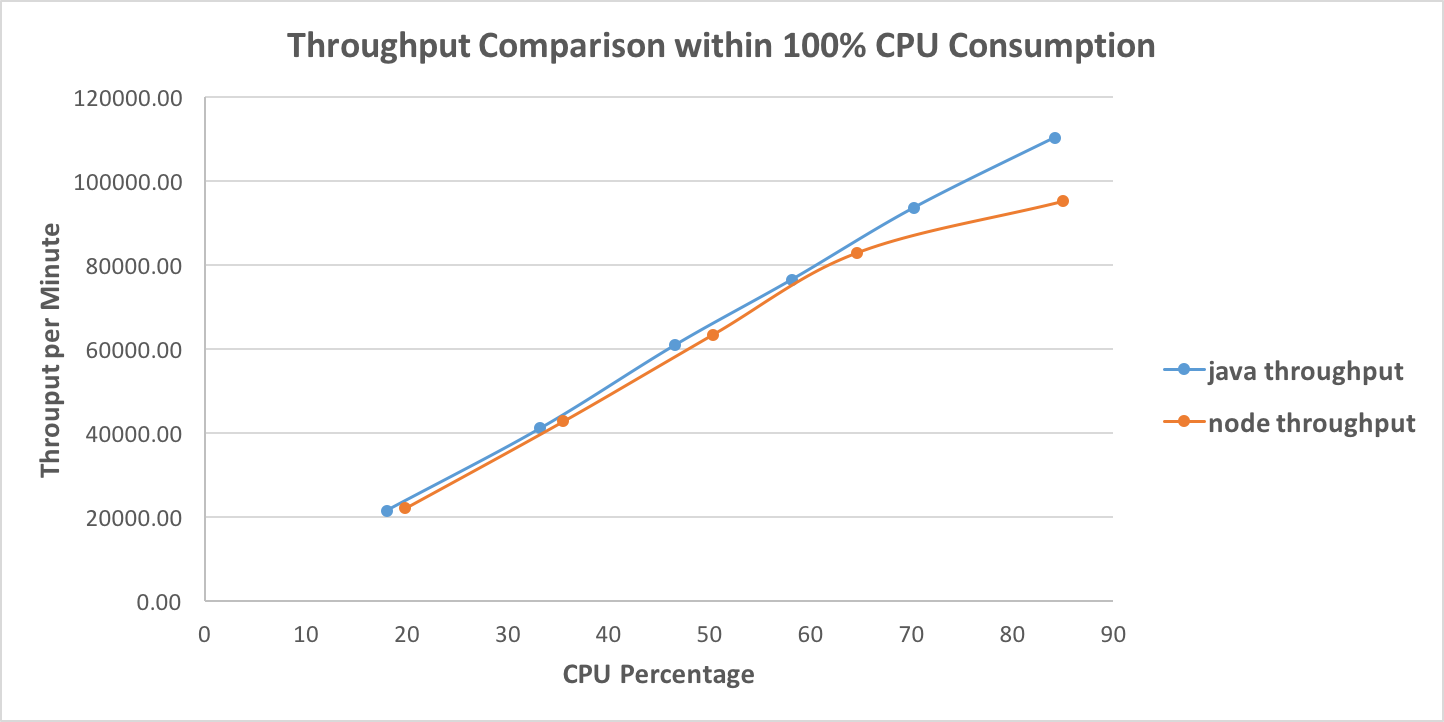
\includegraphics[width=12cm]{cpu-100}
	\caption{Compare throughput under 100 CPU consumption}
	\label{cpu-100}
\end{figure}

\section{Test with real load}
  \todo[inline]{Java scaling}
  \todo[inline]{Node scaling}
